%!TEX root = FreeRtos ARM uController.tex
\subsection{Scheduling}
\label{Scheduling}
Der Scheduler ist die Kernkomponente jedes Echtzeitbetriebssystem Kernels, da er eine quasi parallele Ausführung von Tasks ermöglicht. Eine Task stellt dabei ein ei\-gen\-stän\-di\-ge lauffähige Programmeinheit dar und wird gewöhnlich in einer Schleife ausgeführt. Abhängig vom aktuellen Zustand der Tasks und dem gewählten Schedulingalgorithmus, wählt der Scheduler die nächste Task, die ausgeführt werden soll. Auf einem uProzessor mit einem Kern kann dabei immer nur eine Task zur Zeit ausgeführt werden. Der Vorgang des Task-Wechsels durch den Scheduler wird Kontextwechsel oder Kontextswitch genannt. Der Kontextwechsel ist für eine Task die verdrängt wird nicht erkennbar. Die Task wird bei ihrer aktuell ausgeführten Instruktion unterbrochen und alle nötigen Register under Stack werden durch den Scheduler gesichert. Abbildung \ref{fig:ContextSwitch} zeigt wie eine Task während ihrer Ausführung unterbrochen wird. Nachdem der Scheduler die verdrängte Task wieder zur Ausführung ausgewählt hat, werden alle Register und der Stack wieder hergestellt. Die Task wird danach ab der letzten Instruktion fortgeführt. 
\begin{figure}[ht!]
	\centering
		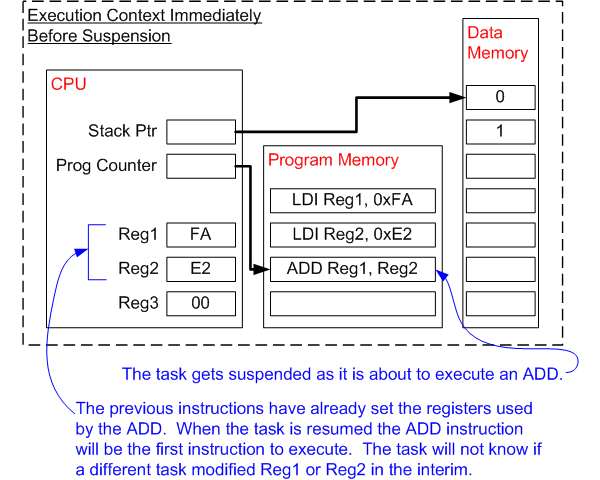
\includegraphics[width=0.4\textwidth]{Pictures/FreeRTOSOrg/ExeContext.png}
	\caption{FreeRTOS Pseudoimplementierung des Context - Switch. Bild-Quelle~\protect\citeA{MasteringFreeRtos} }
	\label{fig:ContextSwitch}
\end{figure}   
Folgende Zu\-stän\-de kann eine FreeRTOS Task annehmen: 
\begin{itemize}
	\item Running
	\item Blocked
	\item Ready
	\item Suspended
\end{itemize}
 Alle Tasks im Ready Zustand sind bereit und warten auf ihre Ausführung durch den Scheduler. Tasks die sich im Blocked Zustand befinden sind nicht bereit und warten auf ein Synchronisations- oder ein Timer Event. Eine Task die vTaskSuspend() aufruft, wird vom Scheduling Vorgang ausgeschlossen und nimmt den Zustand Suspended an. Abbildung \ref{fig:TaskStates} zeigt das Zustandsdiagramm einer FreeRTOS Task. 
\begin{figure}[ht!]
	\centering
		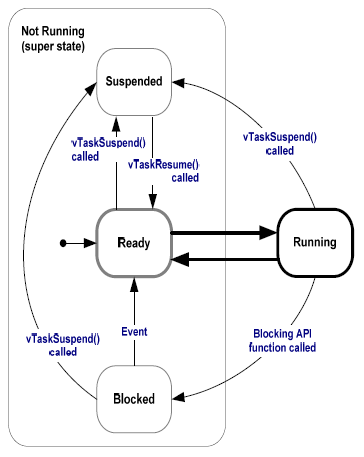
\includegraphics[width=0.3\textwidth]{Pictures/FreeRTOSOrg/taskStates.png}
	\caption{Übersicht aller Task Zustandstransitionen in FreeRTOS. Der Zustandswechsel findet entweder durch den Aufruf einer FreeRTOS API Funktion statt oder aber durch Event z.B. Interrupts, Timer-Events. Der Wechsel in den Zustand Running wird durch den Scheduler bestimmt und ist durch den Schedulingalgorithmus definiert.  Bild-Quelle~\protect\citeA{MasteringFreeRtos}}
	\label{fig:TaskStates}
\end{figure}Welche Task als näch\-stes vom Zustand Ready in den Zustand Running wechselt, wird durch den Scheduler bestimmt. Der Schedulingalgorithmus des Schedulers gibt dabei vor wie diese näch\-ste Task bestimmt wird. Der Scheduling Algorithmus des FreeRTOS Schedulers bietet unterschiedliche Kon\-fi\-gu\-ra\-tions\-mög\-lich\-kei\-ten auf die wir im laufe dieses Abschnittes genauer eingehen werden. Das Scheduling des FreeRTOS Kernels basiert grundsätzlich auf dem Round Robin Algorithmus\cite{9783827373427}. Dabei werden alle lauffähigen Tasks (Ready) gleicher Priorität in einer Liste verwaltet. Jede Task in der Liste erhält ein gewisses Zeitquantum\footnote{Round Robin definiert nicht die Länge des Zeitquantums}, welches bestimmt wie lange einer Task der Prozessor zugeteilt wird. Nach Ablauf des Zeitquantum wird ein Kontextwechsel durchgeführt und die näch\-ste Task in der Liste erhält Prozessorzeit. Die ausgelaufene Task wird durch den Scheduler automatisch hinten an die Liste angefügt. Jede Task in FreeRTOS wird eine gewisse Priorität zugewiesen, daher wird auch für jede Priorität eine eigene Round Robin-Liste geführt. Dieses Verfahren wird auch Priority Scheduling \cite{9783827373427} genannt. Abbildung \ref{fig:PrioList1} veranschaulicht das Ganze. In Listing \ref{lst:nextTask} wird gezeigt wie das Priority Scheduling im FreeRTOS Source Code umgesetzt wurde. 
\begin{figure}[ht!]
	\centering
		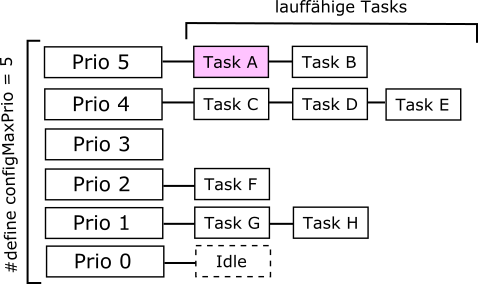
\includegraphics[width=0.3\textwidth]{Pictures/Scheduling/PrioList1.png}
	\caption{Aufbau der Prioritätenliste nach Round Robin in FreeRTOS. Alle aufgeführten Task sind bereit zur Ausführung. Task A wird aktuell durch den Scheduler ausgeführt. Nach dem Ablauf des Zeitquantums, wird A hinter B einsortiert. Die Maximale Priorität wird durch configMaxPrio bestimmt. Die Idle Task wird automatisch durch den Kernel erzeugt und hat immer die niedrigste Priorität. }
	\label{fig:PrioList1}
\end{figure}
\begin{lstlisting}[caption={FreeRTOS Source zur Priroty Task Selection aus Task.c. Alle lauffähigen Task werden in einem Array vewaltet pxReadyTaskLists. Die Listen verwalten sich durch Referenz-Pointer in den TCBs der einzelnen Tasks}, linewidth=8cm,captionpos=b, label=lst:nextTask, float=hbt]
#define taskSELECT_HIGHEST_PRIORITY_TASK(){																									
	UBaseType_t uxTopPriority = uxTopReadyPriority;														
		/* Find the highest priority queue that contains ready tasks. */								
		while(listLIST_IS_EMPTY(&(pxReadyTasksLists[ uxTopPriority ]))){																								
			configASSERT( uxTopPriority );																
			--uxTopPriority;																			
		}																								
		/* listGET_OWNER_OF_NEXT_ENTRY indexes through the list, so the tasks of						
		the	same priority get an equal share of the processor time. */									
		listGET_OWNER_OF_NEXT_ENTRY(pxCurrentTCB, &(pxReadyTasksLists[uxTopPriority]));			
		uxTopReadyPriority = uxTopPriority;																
	} /* taskSELECT_HIGHEST_PRIORITY_TASK */
\end{lstlisting}
Eine Besonderheit ist die Idle Task, diese wird automatisch beim Starten des Schedulers erzeugt. Die Idle Task hat die niedrigste Priorität und wird immer dann ausgeführt, wenn sich keine User-Task im Ready oder Running Zustand befindet. Die Idle Task ist ein Indikator für überschüssige Prozessorzeit. Mittels der Idle-Hook Funktion kann der Idle Task Funktionalität durch den Entwickler hinzugefügt werden. Wie die Idle Task zum Energiesparen genutzt werden kann, wird in Abschnitt \ref{sec:Low Power Modes} gezeigt. Wie bereits weiter oben beschrieben, lässt sich der Scheduling Algorithmus in verschiedenen Modis ausführen. Der Scheduler kann entweder im Cooperative Modus oder im Preemption Modus ausgeführt werden. Welcher Modus vom Scheduler verwendet wird, wird durch das define configUSE\_PREEMPTION in der FreeRTOS config bestimmt. Im Preemtive Modus wird eine aktive Task mit niedriger Priorität sofort von einer Task mit höherer Priorität verdrängt und ein Kontextwechsel wird durchgeführte. Im kooperativen Modus hingegen wird ein Kontextwechsel erst durchgeführt, wenn eine Task den Prozessor explizit durch die Funktion xTaskYield() abgibt. Abbildung \ref{fig:PreVSCo} zeigt den Vergleich beider Modis durch einen beispielhaften Ablauf. Eine weitere Option die sich über das define configUSE\_TIME\_SLICING aktivieren lässt ist das sogenannte Zeitschlitzverfahren. Durch das Zeitschlitzverfahren wird die zugeteilte Prozessorzeit für Task gleicher Priorität gleichmäßig aufgeteilt. Dies geschieht durch Einführung eines festen Tick-Interrupt Intervalls. Bei jedem Tick Interrupt wird der FreeRTOS SysTickHandler aufgerufen. Listing \ref{lst:SysTickS} zeigt die Implementierung des FreeRTOS SysTicks. Der SysTickHandler ist Bestandteil des Schedulers und überprüft bei jeder Ausführung, ob sich eine Task gleicher Priorität im Ready Zustand befindet. Sollte es eine solche Task geben wird ein Kontextwechsel durchgeführt und die Task erhält den Prozessor zugeteilt. Des Weiteren kümmert sich der SysTickHandler um die Verwaltung des TickCount, welcher als Referenz für alle RTOS Timingfunktionen dient. Abbildung \ref{fig:SysTick} zeigt diesen Vorgang nochmal im zeitlichen Verlauf. Die häufigst verwendete Scheduling Algorithmus nennt sich Prioritized Pre-emptive Scheduling with Time Slicing.
\begin{figure}[htb]
	\centering
		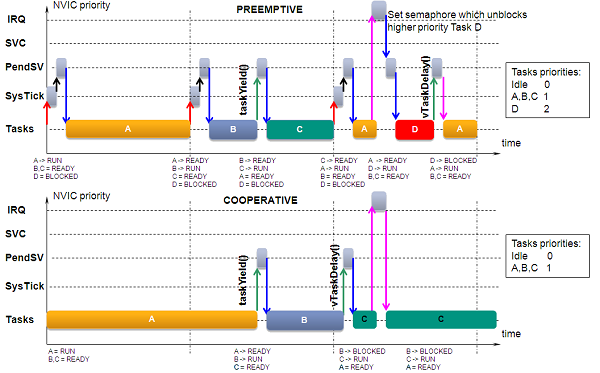
\includegraphics[width=0.5\textwidth]{Pictures/EMCUIT/PreemptiveCooperative.png}
	\caption{Im Co-operative Modus wird der Prozessor von einer Task erst abgegeben, wenn diese explizit taskYield() aufruft. Selbst wenn eine Task mit höhrer Priorität in den Ready Zustand wechselt, läuft die Task mit niedrigerer Priorität weiter. Im Gegensatz dazu steht das Pre-Emptive Scheduling (hier mit Time-Slicing), es unterbricht die laufende Task mit niedriger Priorität sofort, sobald eine Task mit höherer Priorität Ready ist. Bild-Quelle~\protect\citeA{MasteringFreeRtos}}
	\label{fig:PreVSCo}
\end{figure}
\begin{lstlisting}[caption={FreeRTOS Source des SysTickHandlers aus Task.c. Der SysTickHandler verwaltet den TickCount. Der TickCount dient allen Timingfunktionen des RTOS Kernels als Zeitreferenz. Des Weiteren wird bei aktivem Time Slicing überprüft ob ein Kontextwechsel nötig ist. Der Kontext wechsel wir dann ggf. durch den PendSVHandler durchgeführt.}, linewidth=8cm,captionpos=b, label=lst:SysTickS, float=hbt]
void xPortSysTickHandler( void ){
	/* The SysTick runs at the lowest interrupt priority, so when this interrupt
	executes all interrupts must be unmasked.  There is therefore no need to
	save and then restore the interrupt mask value as its value is already
	known. */
	portDISABLE_INTERRUPTS();
	{
		/* Increment the RTOS tick. */
		if( xTaskIncrementTick() != pdFALSE )
		{
			/* A context switch is required.  Context switching is performed in
			the PendSV interrupt.  Pend the PendSV interrupt. */
			portNVIC_INT_CTRL_REG = portNVIC_PENDSVSET_BIT;
		}
	}
	portENABLE_INTERRUPTS();
}
\end{lstlisting}
\begin{figure}[htb]
	\centering
		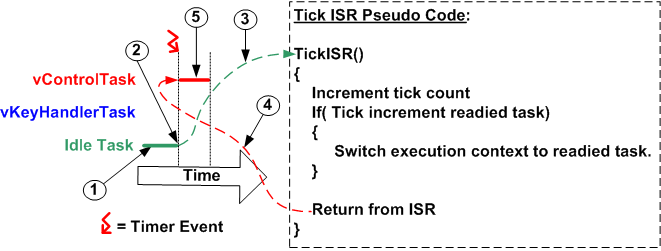
\includegraphics[width=0.4\textwidth]{Pictures/FreeRTOSOrg/TickISR.png}
	\caption{Beispielhafter Ablauf eines SysTickInterrupts.(1) keine User Task ist ready, die Idle Task ist aktiv. (2) SysTickInterrupt. (3) SysTickHandler wird aufgerufen. (4) vControlTask ist ready und ein Kontext wechsel wird durchgeführt. vControlTask hat hier die gleiche Priorität wie die IdleTask. (5)vControlTask wird ausgeführt. Bild-Quelle~\protect\citeA{MasteringFreeRtos}}
	\label{fig:SysTick}
\end{figure}


Listing \ref{lst:TaskExam1} zeigt ein minimal Beispiel einer Task und den Start des Schedulers durch vTaskStartScheduler() in der main function. 
\begin{lstlisting}[caption={Minimal Beispiel für die Definition eine Task. }, linewidth=8cm,captionpos=b, label=lst:TaskExam1, float=hbt]
 void main( void )
 {
	//Task werden oft vor dem Start des Schedulers erzeugt.
	xTaskCreate( vTaskCode,
							"NAME",
							STACK_SIZE,
							NULL,
							tskIDLE_PRIORITY,
							NULL );
   // Scheduler wird gestartet
   vTaskStartScheduler();
   // Hier sollten wir nicht hinkommen, da der Scheduler laeuft.
 }

void vTaskCode( void * pvParameters )
{
    for( ;; ){
        /* Task code wird hier Implementiert
				 z.B. warten auf eine Nachricht*/
    }
		/* Hier sollten wir nicht hinkommen*/
		vTaskDelete( NULL );
}
\end{lstlisting}

